หุ่นยนต์ฮิวมานอยด์ คือ หุ่นยนต์ที่ถูกสร้างขึ้นมาให้มีรูปร่างคล้ายคลึงกับสรีระโครงสร้างของมนุษย์
มักถูกออกแบบขึ้นมาเพื่อจุดประสงค์เฉพาะอย่าง เช่น การใช้เครื่องมือต่างๆของมนุษย์ การอยู่ในสภาพแวดล้อมของมนุษย์
การศึกษาการเคลื่อนไหวของร่ายกายมนุษย์ หรือเพื่อวัตถุประสงค์อื่นๆ โดยทั่วไปแล้ว หุ่นยนต์ฮิวมานอยด์ประกอบไปด้วย 4 ส่วนคือ หัว ลำตัว แขน
และขา แต่การสร้างหุ่นยนต์ฮิวมานอยด์นั้นก็ไม่จำเป็นที่จะต้องมีส่วนประกอบทุกส่วนดังที่กล่าวไป
ในบางครั้งอาจมีเพียงแค่ส่วนบนเท่านั้น ดังรูปที่ \ref{fig:namo} \footnote{คนไทยสุดเจ๋ง!!สร้างหุ่นยนต์ 'น้องนะโม' ทำหน้าที่ต้อนรับแทนคน ทั้งไหว้-พูดหลายภาษา,https://www.thairath.co.th/content/523340}
หุ่นยนต์นะโมจากสถาบันวิทยาการหุ่นยนต์ภาคสนาม เป็นหุ่นยนต์ที่มีส่วนบนเหมือนมนุษย์ แต่มีส่วนล่างเป็นล้อ หรือหุ่นยนต์ฮิวมานอยด์ที่มีเพียงแค่ส่วนล่าง ดังรูปที่ 
\ref{fig:somjook} \footnote{หุ่นยนต์ฮิวมานอยด์เดินสองขาส้มจุก,http://www.fibo.kmutt.ac.th/fiboweb2015/หุ่นยนต์ฮิวมานอยด์เดิน}
หุ่นยนต์ส้มจุก เป็นหุ่นยนต์ฮิวมานอยด์ที่มีเพียงแค่ส่วนขาเท่านั้น หรือหุ่นยนต์ฮิวมานอยด์ที่มีเพียงใบหน้าเหมือนมนุษย์ ดังรูปที่
\ref{fig:sophia} \footnote{ซาอุดิอาราเบียมอบสัญชาติให้กับหุ่นยนต์ครั้งแรกของโลก “Sophia” สาวอัจฉริยะ,https://www.ensurecommunication.com/2017/11/02/ซาอุดิอารเบียมอบสัญชา}
หุ่นยนต์โซเฟีย เป็นแอนดรอยด์ที่มีหน้าตาคล้ายมนุษย์มาก มีตา มีปาก สามารถพูดปฏิสัมพันธ์กับมนุษย์ได้

\begin{figure}[!ht]
    \centering
    \begin{subfigure}[b]{0.3\textwidth}
        \centering
        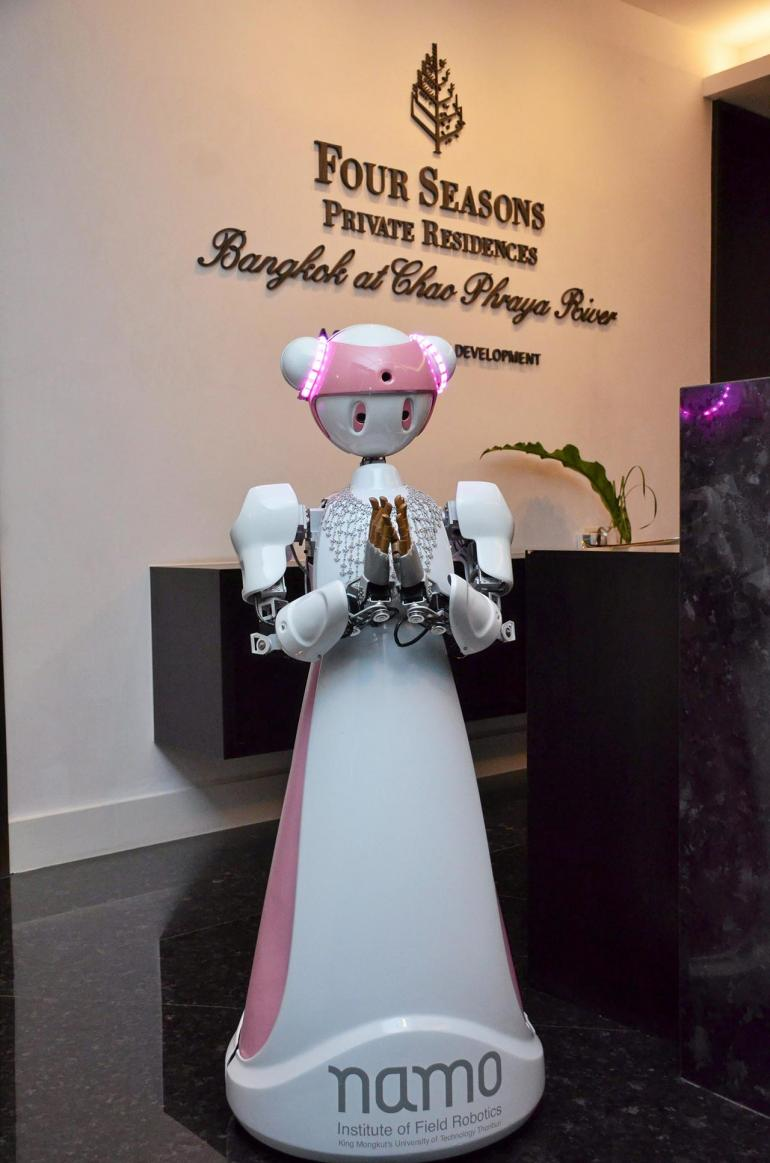
\includegraphics[width=\textwidth]{chapter2/images/namo.jpg}
        \caption{หุ่นยนต์ประชาสัมพันธ์นะโม}
        \label{fig:namo}
    \end{subfigure}
    \hfill
    \begin{subfigure}[b]{0.3\textwidth}
        \centering
        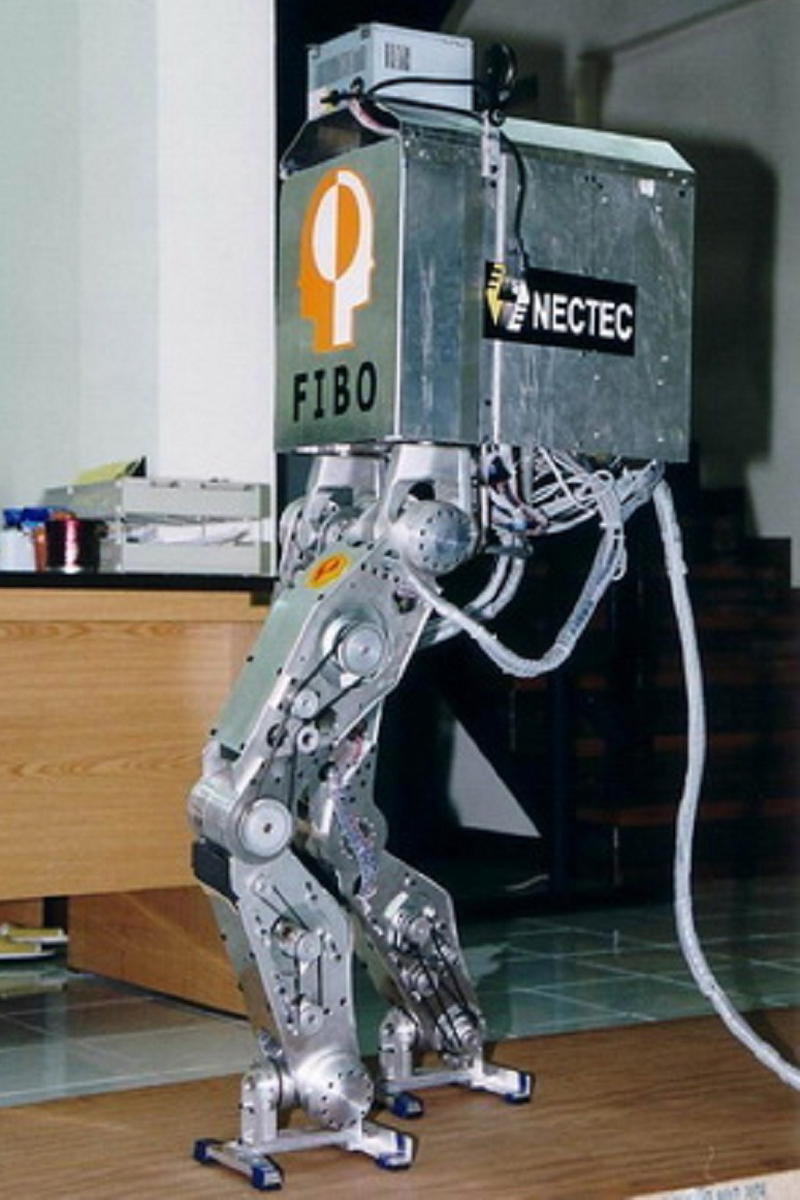
\includegraphics[width=\textwidth]{chapter2/images/ส้มจุก.jpg}
        \caption{หุ่นยนต์เดินสองขาส้มจุก}
        \label{fig:somjook}
    \end{subfigure}
    \hfill
    \begin{subfigure}[b]{0.3\textwidth}
        \centering
        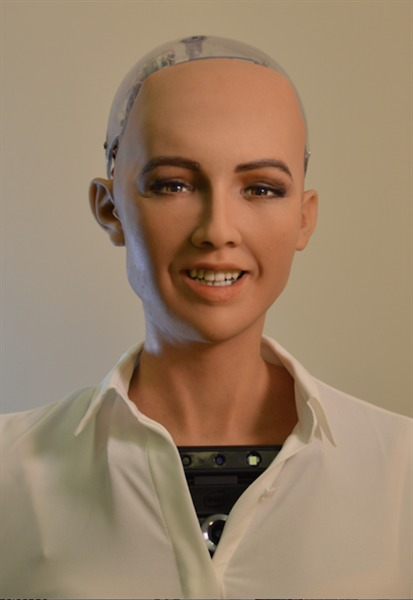
\includegraphics[width=\textwidth]{chapter2/images/โซเฟีย.jpg}
        \caption{หุ่นยนต์แอนดรอยด์โซเฟีย}
        \label{fig:sophia}
    \end{subfigure}
    \caption{แสดงความแตกต่างของหุ่นยนต์ฮิวมานอยด์แต่ละประเภท}
    \label{fig:diff_humanoid}
\end{figure}

\clearpage
งานวิจัยทางด้านหุ่นยนต์ฮิวมานอยด์จากอดีตจนถึงปัจจุบันมีการพัฒนาความสามารถของการเดินของหุ่นยนต์
เช่น เริ่มต้นจากแรกสุดจะเป็นการพัฒนาให้หุ่นยนต์สามารถเดินหน้าได้ ต่อมาก็เพิ่มความสามารถให้หุ่นยนต์สามารถเดินบนพื้นเอียง พื้นขรุขระ
เดินเลี้ยวซ้ายขวา เดินขึ้นลงบันได ฯลฯ เป็นต้น นอกจากนี้ยังมีการพัฒนาปรับปรุงสมดุลของการเดินแบบสองขาอีกด้วย สมดุลของการเดินสามารถแบ่งได้สองแบบหลัก
คือ การเดินแบบสมดุลสถิต และการเดินแบบสมดุลพลวัต งานในยุคแรกนั้นจะพัฒนาให้เดินได้แบบสมดุลสถิต ต่อมาเป็นสมดุลกึ่งพลวัต
และเป็นสมดุลพลวัต การพัฒนาตัวควบคุมการเดินของหุ่นยนต์ จำเป็นที่จะต้องใช้ความรู้ทางด้านกลศาสตร์ค่อนข้างมาก มีการใช้สมการที่มีความซับซ้อน

%\clearpage
%%%%%%%%%%%%%%%%%%%%%%%%%%%%%%%%%%%%%%%%%%%%%%%%%%%%%%%%%%%%%%%%%%%%%%%%%%%%%%%
Zheng และคณะ (1988) พัฒนาหุ่นยนต์สองขาที่สามารถเดินบนพื้นราบได้ ให้สามารถเดินต่อเนื่องไปบนพื้นเอียงได้ด้วย
พื้นเอียงที่ใช้มีลักษณะเป็นพื้นเอียงขึ้น หุ่นยนต์ที่ใช้ในงานนี้มีข้อต่อสะโพก (hip), ข้อเท้า (ankle) และลำตัว (torso) มีเซนเซอร์วัดแรงกด (force sensor)
ติดตั้งอยู่ที่ปลายเท้าและส้นเท้าแต่ละข้างเพื่อใช้วัดตำแหน่งของน้ำหนักโดยรวม (center of gravity) ของหุ่นยนต์ การเดินของงานวิจัยจะพิจารณาเฉพาะการเดินในแนวหน้าหลัง
โดยมีหลักการคือ การเดินบนพื้นเอียงโดยที่หุ่นยนต์ยังเดินในท่าทางเหมือนกับตอนที่เดินบนพื้นราบจะทำให้น้ำหนักโดยรวมของหุ่นยนต์เลื่อนไปข้างหลัง
ดังนั้นการที่หุ่นยนต์ขยับลำตัวไปด้านหน้าจำทำให้น้ำหนักโดยรวมของหุ่นยนต์กลับมาอยู่ตรงกลางของพื้นที่รับน้ำหนักเหมือนเดิม
ซึ่งจะทำให้หุ่นยนต์มีความสมดุลได้ ดั้งนั้นข้อมูลที่ได้จากหน่วยวัดแรงกดที่เท้าจะถูกนำมาคำนวณตลอดการเดินเพื่อใช้ในการปรับเปลี่ยนมุมการขยับของลำตัว
การเดินบนพื้นราบเป็นแบบสมดุลสถิตและการเดินบนพื้นเอียงก็ยังคงเป็นแบบสมดุลสถิตเช่นกัน

Inaba\footnote{Yuki Asano*, Kei Okada and Masayuki Inaba} และคณะ (1995) สร้างหุ่นยนต์เลียนแบบลิง (ape-like biped) ประกอบด้วยสองมือและสองขา มีการเดินแบบสมดุลสถิต
งานวิจัยนี้มีความคิดว่านอกจากการทำให้หุ่นยนต์สองขาเดินได้โดยไม่ล้มแล้ว ควรจะทำหุ่นยนต์ที่สามารถลุกขึ้นเองได้หลังจากที่ล้มแล้วด้วย
ดังนั้นในงานนี้ หุ่นยนต์ถูกพัฒนาให้สามารถเดิน เมื่อล้มแล้วก็สามารถพลิกตัวและลุกขึ้นมาเดินให้ได้

Kun และ Miller\footnote{Modelling of Walking Humanoid Robot With 
Capability of Floor Detection and Dynamic 
Balancing Using Colored Petri Net, Saeid Pashazadeh and Saeed Saeedvand} (1996) ได้นำโครงข่ายประสาทเทียม มาประยุกต์ใช้ในการปรับเปลี่ยนท่าทางการเดินโดยอัตโนมัติของหุ่นยนต์สองขา
การที่หุ่นยนต์สามารถปรับเปลี่ยนท่าทางได้โดยอัตโนมัตินี้มีประโยชน์ทำให้หุ่นยนต์เดินได้บนพื้นผิวหลากหลายลักษณะมากขึ้น
ในงานนี้พิจารณาท้ังสมดุลในแนวหน้าหลัง (sigittal plane) และแนวซ้ายขวา (frontal plane) และการเดินของหุุ่นยนต์เป็นแบบสมดุลพลวัต
หลักการทำงานประกอบด้วยตัวสร้างท่าทางการเดินหนึ่งตัว และตัวปรับท่าทางการเดินทั้งแนวหน้าหลังและซ้ายขวาอีกหนึ่งตัว
โดยค่าการปรับเปลี่ยนนั้นจะได้มาจาก แรงกดที่เท้า ความยาวการก้าวเท้า ความสูงของการยกเท้า เป็นต้น นอกจากนี้
ในปีถัดมาทั้งสิงได้ใช้หลักการที่ใช้ในงานนี้ไปใช้กับการเดินของหุ่นยนต์อีกตัว (Kun and Miller, 1997)

\clearpage
Hirai\footnote{    Kazuo Hirai, (1999) "The Honda humanoid robot: development and future perspective", Industrial Robot: An International Journal, Vol. 26 Issue: 4, pp.260-266, https://doi.org/10.1108/01439919910277431} และคณะ (1998)
พัฒนาหุ่นยนต์ฮิวมานอยด์ ซึ่งตัวหุ่นยนต์มีความคล้ายมนุษย์มาก สามารถเดินได้อย่างราบรื่นคล้ายมนุษย์มากที่สุด
เช่น สามารถเดินได้ในพื้นผิวชนิดต่างๆ เดินได้บนพื้นเอียงขึ้นเอียงลง เดินขึ้นลงบันได้ได้ เดินเข็นรถได้ เป็นต้น การเดินในทุกสถานการณ์เป็นการเดินแบบสมดุลพลวัต
หุ่นยนต์สามารถเดินได้ด้วยความเร็วสูงสุด 4.7 กิโลเมตรต่อชั่วโมง หุ่นยนต์ประกอบไปด้วย แขนข้างละ 9 องศาอิสระ ขาข้างละ 6 องศาอิสระ
ที่บริเวณหัวมีกล้องติดตั้งอยู่ 4 ตัว นอกจากนี้ยังมีอุปกรณ์ที่ใช้ในการรักษาสมดุลอื่นๆ อีกได้แก่ IMU ที่ติดตั้งบริเวณลำตัว และ Force sensor ที่ติดที่เท้าทั้งสองข้าง
\begin{figure}[!ht]
    \centering
    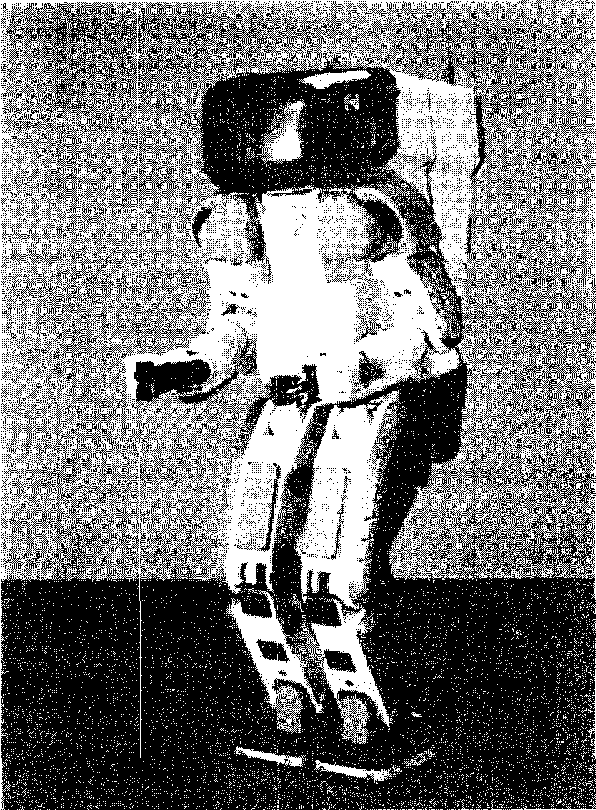
\includegraphics[width=0.22\textwidth]{chapter2/images/honda_asimo.png}
	\caption{Honda asimo โดย Kazou Hirai}
    \label{fig:humanoid_asimo}
\end{figure}



%\clearpage
%%%%%%%%%%%%%%%%%%%%%%%%%%%%%%%%%%%%%%%%%%%%%%%%%%%%%%%%%%%%%%%%%%%%%%%%%%%%%%%
องค์ประกอบของหุ่นยนต์ทั่วไปจะประกอบไปด้วยกระบวนการตอบสนองต่างๆที่เป็นระบบ
ซึ่งเราสามารถจำแนกกาออกเป็นส่วนหลักๆได้สามส่วนคือ ส่วนการรับรู้ ส่วนการประมวลผล
และส่วนการขับเคลื่อน ทั้งหมดเมื่อนำมารวมเข้าด้วยกันแล้ว เราสามารถที่จะควบคุมการทำงานของหุ่นยนต์ฮิวมานอยด์ได้

\subsubsection*{การรับรู้ของหุ่นยนต์ฮิวมานอยด์}
การรับรู้ของหุ่นยนต์ฮิวมานอยด์นั้นมีความยากมากกว่าหุ่นยนต์ชนิดอื่นๆเนื่องจาก หุ่นยนต์ฮิวมานอยด์เกิดจากการนำก้านต่อหลายๆชิ้นเข้ามาเชื่อมต่อกันด้วยข้อต่อ
ทำให้หุ่นยนต์ฮิวมานอยด์สามารถเคลื่อนไหวเป็นท่าทางต่างๆได้ และไม่มีส่วนใดถูกตรึงยึดติดกับพื้นโลก ซึ่งทำให้เราไม่สามารถที่จะอ้างอิงท่าทางของหุ่นยนต์ได้
จึงจำเป็นที่จะต้องเพิ่มส่วนของการรับรู้เข้าไปเพื่อช่วยแก้ปัญหาในส่วนนี้ เซนเซอร์ที่เพิ่มเข้าไปมีหลากหลายชนิด และแต่ละชนิดก็ทำหน้าที่แตกต่างกัน
ยกตัวอย่างเช่น เซนเซอร์เอนโคดเดอร์ที่ใช้สำหรับอ่านสถานะตำแหน่งและความเร็วของข้อต่อได้ เซนเซอร์หน่วยวัดความเฉื่อยที่ใช้สำหรับหามุมเอียงของตัวหุ่นยนต์
และเซนเซอร์วัดแรงที่ฝ่าเท้าที่จะช่วยในการบอกว่าเท้าของหุ่นยนต์สัมผัสพื้นหรือไม่ เป็นต้น

\clearpage
\subsubsection*{การประมวลผลของหุ่นยนต์ฮิวมานอยด์}
ในปัจจุบันนี้หน่วยประมวลผลของหุ่นยนต์ฮิวมานอยด์มีประสิทธิภาพเพียงพอต่อการควบคุมหุ่นยนต์ฮิวมานอยด์แบบเรียลไทม์ได้
การประมวลผลนั้นสามารถที่จะแบ่งออกเป็นหลายๆส่วนได้ ยกตัวอย่างเช่น

\subparagraph*{หุ่นยนต์ฮิวมานอยด์ Thormang}
ได้แบ่งตัวประมวลผลเป็นตัวประมวลควบคุมสำหรับสั่งการตัวขับเคลื่อน ตัวประมวลผลควบคุมสำหรับอ่านสถานะตัวรับรู้ และตัวประมวลผลควบคุมภายนอกสำหรับคำนวณท่าทางการเดินและการวางเท้า
\subparagraph*{หุ่นยนต์ฮิวมานอยด์ Robotis OP3}
ได้แบ่งตัวประมวลผลเป็นตัวประมวลผลระดับสูงสำหรับคำณวณท่าทางการเคลื่อนไหว และตัวประมวลผลระดับล่างสำหรับสั่งการตัวขับเคลื่อนและอ่านสถานะตัวรับรู้
\subparagraph*{หุ่นยนต์ฮิวมานอยด์ Poppy}
ไม่ได้แบ่งตัวประมวลผล แต่ใช้เพียงตัวเดียวในการสั่งการตัวขับเคลื่อน อ่านสถานะตัวรับรู้ และประมวลผลการคำนวณทั้งหมด

นอกจากการประมวลผลและควบคุมแล้ว ยังรวมไปถึงหน่วยแสดงผลที่สามารถนำค่าสถานะต่างๆจากหุ่นยนต์ฮิวมานอยด์ออกไปสร้างเป็นกราฟ หรือแบบจำลองสามมิติได้อีกด้วย

\subsubsection*{การขับเคลื่อนของหุ่นยนต์ฮิวมานอยด์}
การที่หุ่นยนต์ฮิวมานอยด์สามารถที่จะทำท่าทางต่างๆได้นั้น เกิดจากการเปลี่ยนแปลงตำแหน่งของข้อต่อ ดั้งนั้นการที่หุ่นยนต์จะขับเคลื่อนข้อต่อได้นั้น
ก็จึงจำเป็นที่จะต้องมีตัวขับเคลื่อนที่ข้อต่อ โดยทั่วไปแล้วเราจะติดมอเตอร์เซอร์โวไว้ที่ตำแหน่งเดียวกับข้อต่อเลย เหตุผลที่นิยมใช้มอเตอร์เซอร์โวเนื่องจาก
เซอร์โวสามารถที่จะควบคุมตำแหน่งและความเร็วได้
